\section{积分与极限}
\label{sec:integral-limits}

函数列逐点收敛时，积分未必随之收敛：前面的例子已经显示，逐点趋于零的函数可以保持积分为一。本节固定测度$\mu$，研究函数列或函数项级数在什么条件下允许交换积分与极限。各小节按可以核查的条件组织：非负且递增；只有非负；所有项受同一个可积函数控制；各项绝对积分之和有限；以及有限测度上的一致收敛。每个条件下给出相应的定理和使用方式，并用反例说明去掉条件后哪里出错。测度本身随参数变化时积分怎样收敛，是另一类问题，留待后文讨论测度序列的收敛时处理。

\subsection{非负递增条件下的极限交换}
\label{sec:integral-limits-monotone}

\paragraph{递增列}
第~\ref{sec:integral-mct}小节的单调收敛定理（定理~\ref{thm:integral-monotone-convergence}）已经回答了最简单的情形：若$0\le f_1\le f_2\le\cdots$可测且逐点趋于$f$，则$\int f_n\to\int f$，共同结果可以是$+\infty$。核查条件时只需确认两点：各项非负，且逐点递增（允许在零测集外成立）。不需要任何可积性，这是它与后面几种条件的主要区别。下面把它用于两种常见操作，它们都归结为同一个非负递增条件。

\begin{theorem}[非负级数的逐项积分与递增区域]
\label{thm:integral-series-nonnegative}
\begin{enumerate}
 \item 设$g_1,g_2,\dots:X\to[0,+\infty]$可测，则$\int_X\sum_{k=1}^\infty g_k\,\mathrm d\mu=\sum_{k=1}^\infty\int_Xg_k\,\mathrm d\mu$。
 \item 设$f\ge0$可测，$E_1\subseteq E_2\subseteq\cdots$可测，$E=\bigcup_nE_n$，则$\int_{E_n}f\,\mathrm d\mu\to\int_Ef\,\mathrm d\mu$。
 \item 设$f\ge0$可测，则$\nu(E)=\int_Ef\,\mathrm d\mu$定义$(X,\mathcal A)$上的测度。
\end{enumerate}
\end{theorem}

\begin{proof}
第1条：部分和$S_N=\sum_{k\le N}g_k$非负、递增，逐点趋于$\sum_kg_k$；由非负积分的加法$\int S_N=\sum_{k\le N}\int g_k$，再用单调收敛定理。第2条：$f\mathbf 1_{E_n}\uparrow f\mathbf 1_E$，用单调收敛定理。第3条：$\nu(\varnothing)=0$；若$E_k$两两不交，则$f\mathbf 1_{\bigcup_kE_k}=\sum_kf\mathbf 1_{E_k}$，由第1条得可数可加性。
\end{proof}

第3条中的测度$\nu$把每个区域上的累计值记录下来，它在$\mu$-零测集上取零（引理~\ref{lem:integral-nonnegative-basic}第3条）。反过来，哪些测度能写成这种形式，是第~\ref{chap:densities-change-of-measure}章的主题。

\paragraph{两个计算}
在$(0,1)$上，$-\log(1-x)/x=\sum_{k\ge1}x^{k-1}/k$，各项非负。由$\int_0^1x^{k-1}/k\,\mathrm dx=1/k^2$与第1条，
\[
 \int_{(0,1)}\frac{-\log(1-x)}x\,\mathrm dx=\sum_{k=1}^\infty\frac1{k^2}\le1+\sum_{k\ge2}\frac1{k(k-1)}=2,
\]
所以这个在$x\to1$处无界的函数可积（级数的值为$\pi^2/6$，这一经典结果此处用不到）。对递增区域，取$E_n=[1,n]$，$\int_{E_n}x^{-2}\,\mathrm dx=1-1/n\to1$，这就是上一节反常积分结论的来源。两种操作中，若结果为$+\infty$，等式同样成立：$\sum_{k\ge0}x^k=1/(1-x)$在$[0,1)$上逐项积分，左边$\int_0^1\mathrm dx/(1-x)=+\infty$，右边$\sum_k1/(k+1)=+\infty$。

\subsection{非负条件下的积分下界}
\label{sec:integral-limits-fatou}

\paragraph{Fatou引理}
当非负函数列不再递增时，可以先构造一列递增的下界。尾部下确界$g_n=\inf_{k\ge n}f_k$随$n$递增，并趋于$\liminf_nf_n$；对它用单调收敛定理，就得到下面的不等式。

\begin{lemma}[Fatou引理]
\label{lem:integral-fatou}
设$f_1,f_2,\dots:X\to[0,+\infty]$可测，则
\[
 \int_X\liminf_{n\to\infty}f_n\,\mathrm d\mu\le\liminf_{n\to\infty}\int_Xf_n\,\mathrm d\mu.
\]
这一结论称为\term{Fatou引理}（Fatou's lemma）。
\end{lemma}

\begin{proof}
令$g_n=\inf_{k\ge n}f_k$，由定理~\ref{thm:measure-limits}可测，$0\le g_1\le g_2\le\cdots$，且$\sup_ng_n=\liminf_nf_n$。对每个$k\ge n$有$g_n\le f_k$，故$\int g_n\le\int f_k$，从而$\int g_n\le\inf_{k\ge n}\int f_k$。由单调收敛定理，
\[
 \int\liminf_nf_n=\lim_n\int g_n\le\lim_n\inf_{k\ge n}\int f_k=\liminf_n\int f_n.
\]
\end{proof}

引理不要求$f_n$逐点收敛，也不要求可积；它只给出“先取极限再积分”的一个下界。若$f_n$逐点收敛到$f$，结论读作$\int f\le\liminf\int f_n$：极限函数的积分不会超过积分的下极限，但可能更小。

\paragraph{丢失的积分质量}
在实轴上取$f_n=\mathbf 1_{[n,n+1]}$。固定$x$，当$n>x$时$f_n(x)=0$，所以$f_n$逐点趋于$0$，左边为$0$；而每个$\int f_n\,\mathrm d\lambda=1$，右边为$1$，不等式严格成立。图~\ref{fig:integral-escaping-mass}(a)显示，单位质量整体向远处平移，每个固定的点最终都看不到它，点态极限因此丢失了全部积分质量。

\begin{figure}[!htbp]
 \centering
 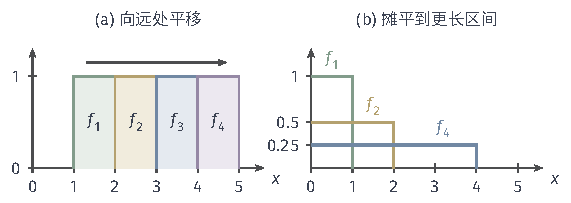
\includegraphics[width=96.629mm]{figures/02-abstract-mathematics/01-metric-and-measure/tikz/c3-escaping-mass/figure.pdf}
 \caption{积分质量从点态极限中丢失的两种方式。(a)$f_n=\mathbf 1_{[n,n+1]}$（$n=1,2,3,4$）向远处平移，逐点趋于零而每项积分为$1$。(b)$f_n=n^{-1}\mathbf 1_{[0,n]}$（$n=1,2,4$）摊平到越来越长的区间，$\sup|f_n|=1/n$一致趋于零而每项积分仍为$1$。}
 \label{fig:integral-escaping-mass}
\end{figure}

非负性也不能去掉：把上例换成$-f_n$，点态极限的积分为$0$，而$\liminf\int(-f_n)=-1$，不等式反向。只有非负性时，通常只能得到下界；要把不等式变为等式，需要阻止质量逃逸。下一小节的统一控制条件正是为此而设。

\subsection{可积控制条件下的极限交换}
\label{sec:integral-limits-dominated}

\paragraph{控制收敛定理}
若所有$|f_n|$都被同一个可积函数$g$压住，质量就无处可逃：$g$本身的积分有限，任何试图跑到远处或集中到窄峰的质量都受$g$在那里的取值约束。证明的办法是对非负函数$2g-|f_n-f|$应用Fatou引理。

\begin{theorem}[控制收敛定理]
\label{thm:integral-dominated-convergence}
设$f_n$、$f$是实值或复值可测函数，$g\ge0$可积，满足：$f_n\to f$ $\mu$-几乎处处；对每个$n$，$|f_n|\le g$ $\mu$-几乎处处。则$f$可积，
\[
 \lim_{n\to\infty}\int_X|f_n-f|\,\mathrm d\mu=0,\qquad\lim_{n\to\infty}\int_Xf_n\,\mathrm d\mu=\int_Xf\,\mathrm d\mu.
\]
这一结论称为\term{控制收敛定理}（dominated convergence theorem），$g$称为控制函数。
\end{theorem}

\begin{proof}
\emph{合并例外集。}按定义，收敛与每个不等式$|f_n|\le g$各在某个零测集外成立；再加上$\{g=+\infty\}$，它由引理~\ref{lem:integral-nonnegative-basic}第5条是零测集。这些例外集只有可数个，其并$N$仍是零测集。把$f_n,f,g$都乘以$\mathbf 1_{X\setminus N}$，函数仍可测，各积分不变（引理~\ref{lem:integral-nonnegative-basic}第3条），而现在收敛与控制在每一点成立，$g$处处有限。

\emph{极限函数可积。}由$|f_n|\le g$及逐点收敛，$|f|\le g$，故$f$可积。

\emph{应用Fatou引理。}$|f_n-f|\le|f_n|+|f|\le2g$，所以$h_n=2g-|f_n-f|$是非负可测函数，且逐点趋于$2g$。由Fatou引理，
\[
 \begin{aligned}
  \int2g&\le\liminf_n\int h_n=\liminf_n\Bigl(\int2g-\int|f_n-f|\Bigr)\\
  &=\int2g-\limsup_n\int|f_n-f|,
 \end{aligned}
\]
其中第一个等号用了可积函数的线性，所有量都有限。消去有限数$\int2g$，得$\limsup_n\int|f_n-f|\le0$，即$\int|f_n-f|\to0$。最后由绝对值估计，$\bigl|\int f_n-\int f\bigr|\le\int|f_n-f|\to0$。
\end{proof}

证明中“消去$\int2g$”一步要求它有限，这正是控制函数必须可积的原因；而合并例外集只用到可数个零测集之并仍是零测集。积分绝对误差$\int|f_n-f|\,\mathrm d\mu$在这里只是一个数，它趋于零比积分本身收敛更强；把它作为函数空间的距离来研究，属于后面讨论$L^1$空间时的内容。

\paragraph{一个可控与一个不可控的例子}
在$[0,+\infty)$上令
\[
 f_n(x)=(1-x/n)^n\mathbf 1_{[0,n]}(x).
\]
对固定的$x$，当$n>x$时$f_n(x)=(1-x/n)^n\to\mathrm e^{-x}$。又由$\log(1-t)\le-t$（$0\le t<1$），$0\le f_n(x)\le\mathrm e^{-x}$，而$\mathrm e^{-x}$在$[0,+\infty)$上可积，积分为$1$（第~\ref{sec:integral-improper}小节）。控制收敛定理给出$\int_0^n(1-x/n)^n\,\mathrm dx\to1$；直接计算，代换$u=1-x/n$得$\int_0^n(1-x/n)^n\,\mathrm dx=n\int_0^1u^n\,\mathrm du=n/(n+1)$，确实趋于$1$。

反过来，在$[0,1]$上取$f_n=n\mathbf 1_{(0,1/n)}$，各项可积且积分恒为$1$，并在每一点趋于$0$，但积分的极限$1$不等于$0$。定理失效是因为找不到可积的控制函数：任何控制函数都不小于上包络$h=\sup_nf_n$，而在$[\frac1{n+1},\frac1n)$上$h=n$，故$h(x)\ge1/x-1$，$\int_0^1(1/x-1)\,\mathrm dx=+\infty$。图~\ref{fig:integral-dominating-envelope}对比了两种情形：(a)中$f_n=x^n$都在可积的常数$1$之下，$\int x^n=1/(n+1)\to0$与点态极限（几乎处处为$0$）的积分一致；(b)中窄而高的矩形把质量集中到原点附近，它们的上包络已不可积。

\begin{figure}[!htbp]
 \centering
 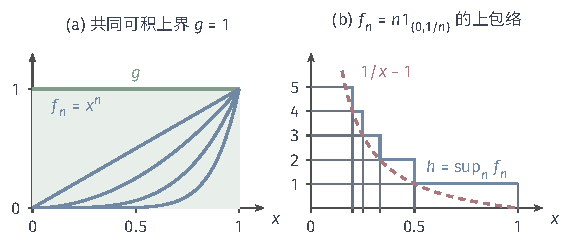
\includegraphics[width=96.633mm]{figures/02-abstract-mathematics/01-metric-and-measure/tikz/c3-dominating-envelope/figure.pdf}
 \caption{控制函数与上包络。(a)$[0,1]$上$f_n=x^n$（$n=1,2,4,8$）都位于可积函数$g=1$之下，积分$1/(n+1)\to0$。(b)$f_n=n\mathbf 1_{(0,1/n)}$（灰色，$n=1,\dots,5$）积分恒为$1$；上包络$h=\sup_nf_n$（蓝色阶梯）在$[\frac1{n+1},\frac1n)$上等于$n$，不小于$1/x-1$（红色虚线），后者在$(0,1)$上积分为$+\infty$，所以不存在可积的控制函数。}
 \label{fig:integral-dominating-envelope}
\end{figure}

\paragraph{函数项级数}
对级数$\sum_kf_k$，把部分和记为$S_N=\sum_{k\le N}f_k$。若$S_N$几乎处处收敛，并且所有$|S_N|$受同一个可积函数控制，就对部分和应用定理，得到$\int\sum_kf_k=\sum_k\int f_k$。需要控制的是部分和，不是单项：在$[0,1]$上取$f_k=\frac1k\mathbf 1_{[0,1]}$，每一项都不超过可积函数$1$，部分和却是调和级数的部分和，逐点发散。

交错几何级数是一个部分和受控而单项绝对积分不可和的例子。在$[0,1)$上，$S_N(x)=\sum_{k=0}^N(-x)^k=\frac{1-(-x)^{N+1}}{1+x}$，满足$|S_N|\le2$，并逐点收敛到$1/(1+x)$。常数$2$在$[0,1)$上可积，所以
\[
 \sum_{k=0}^\infty\frac{(-1)^k}{k+1}=\sum_{k=0}^\infty\int_0^1(-x)^k\,\mathrm dx=\int_0^1\frac{\mathrm dx}{1+x}=\log2.
\]
这同时求出了第~\ref{sec:integral-discrete-sums}小节交错调和级数按原次序的和。注意每一项的绝对积分为$1/(k+1)$，对$k$求和得$+\infty$，下一小节的条件在这里并不成立；控制部分和是比它更细的论证。

\subsection{绝对积分可和条件下的逐项积分}
\label{sec:integral-limits-absolute-series}

\paragraph{逐项检查的条件}
构造部分和的控制函数往往要先知道级数的和。下面的条件只需逐项计算积分，并且自动提供控制函数与截断误差。

\begin{theorem}[绝对积分可和时的逐项积分]
\label{thm:integral-absolute-series}
设$f_1,f_2,\dots$是实值或复值可测函数，且$\sum_{n=1}^\infty\int_X|f_n|\,\mathrm d\mu<+\infty$。则$\sum_n|f_n(x)|<+\infty$对$\mu$-几乎所有$x$成立；在这些点上令$f(x)=\sum_nf_n(x)$，其余点令$f(x)=0$，则$f$可积，
\[
 \int_Xf\,\mathrm d\mu=\sum_{n=1}^\infty\int_Xf_n\,\mathrm d\mu,\qquad\int_X\Bigl|f-\sum_{n\le N}f_n\Bigr|\,\mathrm d\mu\le\sum_{n>N}\int_X|f_n|\,\mathrm d\mu.
\]
这种交换称为\term{逐项积分}（termwise integration）。
\end{theorem}

\begin{proof}
令$G=\sum_n|f_n|$。由定理~\ref{thm:integral-series-nonnegative}第1条，$\int G=\sum_n\int|f_n|<+\infty$，再由引理~\ref{lem:integral-nonnegative-basic}第5条，$G$几乎处处有限。在可测集$\{G<+\infty\}$上级数绝对收敛，因而收敛；$f$是部分和的逐点极限乘以该集合的示性函数，可测。部分和$S_N$满足$|S_N|\le G$，$G$可积，由控制收敛定理得$\int S_N\to\int f$，即$\sum_{n\le N}\int f_n\to\int f$。余项估计：在$\{G<+\infty\}$上$|f-S_N|\le\sum_{n>N}|f_n|$，对右端再用定理~\ref{thm:integral-series-nonnegative}第1条。
\end{proof}

条件$\sum_n\int|f_n|<+\infty$同时完成了三件事：说明级数几乎处处绝对收敛，给出控制函数$G$，并给出截断误差的上界。它比上一小节对部分和的控制要求更强，但更容易验证。

\paragraph{一个带误差的计算}
在$(0,1)$上，$\frac{\log(1+x)}x=\sum_{n\ge1}(-1)^{n+1}\frac{x^{n-1}}n$。各项满足$\int_0^1\bigl|\frac{x^{n-1}}n\bigr|\,\mathrm dx=\frac1{n^2}$，其和有限，定理适用：
\[
 \int_0^1\frac{\log(1+x)}x\,\mathrm dx=\sum_{n=1}^\infty\frac{(-1)^{n+1}}{n^2}.
\]
保留前$N$项时，误差不超过$\sum_{n>N}\frac1{n^2}\le\sum_{n>N}\frac1{n(n-1)}=\frac1N$。例如取前$10$项，积分值与$\sum_{n\le10}(-1)^{n+1}/n^2$之差不超过$0.1$；实际误差还要小得多，这里的上界只用到逐项的绝对积分。

\subsection{有限测度与一致收敛条件下的极限交换}
\label{sec:integral-limits-uniform}

\paragraph{统一误差乘以总测度}
卷1在闭区间上证明过：一致收敛的黎曼可积函数列可以逐项积分，关键是“统一误差乘以区间长度”。在一般测度空间上，区间长度换成总测度，论证同样成立。

\begin{theorem}[有限测度上的一致收敛]
\label{thm:integral-uniform-finite}
设$\mu(X)<+\infty$，$f_n$是实值或复值可积函数，且在$X$上一致收敛到$f$，即$\sup_X|f_n-f|\to0$。则$f$可积，并且
\[
 \int_X|f_n-f|\,\mathrm d\mu\le\mu(X)\sup_X|f_n-f|\to0,\qquad\int_Xf_n\,\mathrm d\mu\to\int_Xf\,\mathrm d\mu.
\]
\end{theorem}

\begin{proof}
$f$是可测函数列的逐点极限，可测。取$N$使$\sup_X|f-f_N|\le1$，则$|f|\le|f_N|+1$，而$|f_N|$与常数$1$在有限测度空间上都可积，故$f$可积。对每个$n$，$|f_n-f|\le\sup_X|f_n-f|$，积分后得估计式；再由绝对值估计得积分收敛。
\end{proof}

定理要求每一项都可积，这在证明的最后一步使用：估计$\bigl|\int f_n-\int f\bigr|$时，$\int f_n$必须是有限数。例如在$[0,1]$上，$\sum_{k\le n}x^k/k!$一致收敛到$\mathrm e^x$，于是$\int_0^1\mathrm e^x\,\mathrm dx=\lim_n\sum_{k\le n}\frac1{(k+1)!}=\mathrm e-1$。

\paragraph{无限测度上的反例}
有限测度不可省略。在$[0,+\infty)$上取$f_n=n^{-1}\mathbf 1_{[0,n]}$，则$\sup|f_n|=1/n\to0$，函数列一致收敛到$0$，而每个$\int f_n\,\mathrm d\lambda=1$。图~\ref{fig:integral-escaping-mass}(b)显示，质量没有集中，而是摊平到越来越长的区间上；统一误差$1/n$乘以支撑区间的长度$n$恰好保持为$1$。与(a)的平移相比，这里连逐点误差的上确界都趋于零，失败完全来自总测度无限。

本节五类条件各有用途：单调收敛不要求可积，允许结果为无穷；Fatou引理只要求非负，给出下界；控制收敛要求一个共同的可积上界，是最常用的一般工具；绝对积分可和便于逐项检查并附带误差估计；有限测度上的一致收敛最容易验证，但适用范围最窄。图~\ref{fig:integral-escaping-mass}与图~\ref{fig:integral-dominating-envelope}中的反例分别对应质量逃逸到远处、摊平到无限测度和集中到窄峰三种失效方式。
